\section{Models testing}
\label{sec:models_testing}
% En esta última sección, se analizarán los resultados de las predicciones obtenidas utilizando la combinación M2 (bert\_base\_uncased + LinearSVC), que fue la que en terminos generales, con un $\sim$ 100\% para el grupo de entrenamiento y un 98\% para el grupo de testeo, entrego las mejores precisiones. A diferencia de la sección anterior (Sección ), en donde se generaron distribuciones de predicciones sobre las 9003 preguntas pre-procesadas (Subsección ), en esta etapa, el modelo será alimentado con el total de preguntas del conjunto de datos VizWiz-VQA sin filtrar. Nuevamente, el conjunto de testeo será dejado a un lado, ya que no posee respuestas asociadas y por ende categorías para poder contrastar resultados.
In this last section, the results of the predictions obtained using the M2 combination (bert\_base\_uncased + LinearSVC) will be analyzed, which was the one that in general terms, with 98\% precision in the testing group, delivered the best results. Unlike the previous section, Section (\ref{sec:classifier}), where prediction distributions were generated on the 9003 pre-processed questions, Figure (\ref{fig:dist_m2}); at this stage, the model was fed with all questions from the unfiltered VizWiz-VQA dataset. Again, the test set will be left aside, since it does not have associated answers and therefore categories to be able to contrast results.

% La Figura (\ref{fig:mco_mod2}), muestra la matriz de confusión entre las nuevas clases: 
% \emph{choice}, \emph{color}, \emph{explication}, \emph{ident}, \emph{observation}, \emph{ocr}, \emph{rel\_ident}, \emph{yes\_no}, y las antiguas categorías: \emph{yes/no, unanswerable, other, number}; sobre el total de 24842 preguntas. Notar que cada celda de la matriz, representa que porcentaje de la antigua categoria ('answer\_type') fué clasificada con la predicción indicada inmediatamente debajo, sobre el eje horizontal.
Figure (\ref{fig:mco_mod2}), shows the confusion matrix between the new classes:
\emph{choice}, \emph{color}, \emph{explanation}, \emph{ident}, \emph{observation}, \emph{ocr}, \emph{rel\_ident}, \emph{yes\_no }, and the old categories: \emph {yes/no, unanswerable, other, number}; over the total of 24842 questions. Note that each cell of the matrix represents what percentage of the old category ('Answer Type') was classified with the prediction indicated immediately below, on the horizontal axis.

\begin{figure}[ht!]
    \centering
    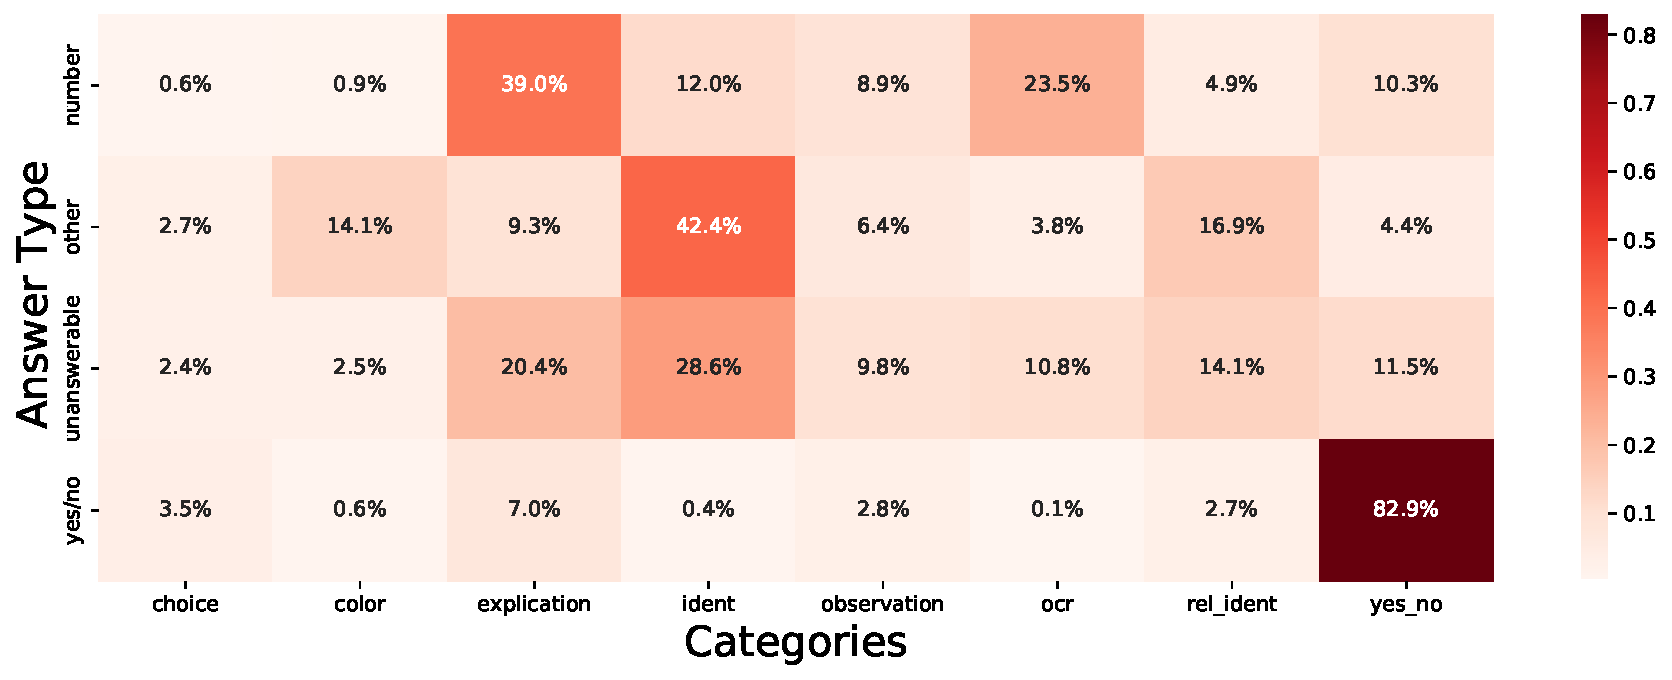
\includegraphics[width=\linewidth]{images/testing/mc_m2_v2.pdf}
\caption{Confusion matrix of M2 combination: 'bert\_base\_uncased + LinearSVC', over full VizWiz-VQA dataset.}
\label{fig:mco_mod2}
\end{figure}


% Dos observaciones naturales que inicialmente se pueden realizar sobre la matriz de la Figura (), son sobre las clases 'number' y 'yes/no'; únicas clases originales descriptivas del conjunto. 
% Si miramos la clase 'yes/no', podemos ver que el $\sim$82\% de las preguntas mantuvieron su categorización, lo que da una muy buena primera impresión, respecto de la confianza de nuestro clasificador.
% Al analizar la clase 'number', vemos que las predicciones se centran con el $\sim$23\% y el $\sim$39\% en las predicciones 'ocr' y 'explication' respectivamente. A pesar de que pueda a primera vista parecer erróneo, esto es muy consistente, ya preguntas del tipo: \emph{'How many cups are there?', How many doors? or 'How many fingers in this image?'} requieren contar objetos, y no necesitan capacidades de reconocimiento optico de caracteres como: \emph{'What is the number on this barcode?', 'What is the oven temperature setting?' or 'What is the second number?'}.
Two natural observations that can initially be made on the matrix of Figure (\ref{fig:mco_mod2}), are on the classes 'number' and 'yes/no'; unique descriptive original classes of the set. If we look at the 'yes/no' class, we can see that the $\sim$82\% of the questions maintained their categorization, which gives a very good first impression, regarding the confidence of our classifier.
When analyzing the class 'number', we see that the predictions are centered with the $\sim$23\% and the $\sim$39\% in the predictions `ocr' and `explication' respectively. Although it may seem wrong at first glance, this is quite consistent. Questions such as: \emph{`How many cups are there?', `How many doors?' or `How many fingers in this image?'} require counting objects, and do not need optical character recognition capabilities such as: \emph{`What is the number on this barcode?', `What is the oven temperature setting?' or `What is the second number?'}.

% Poder descubrir la conformación de la clase 'other', fue una de las principales motivaciones que llevaron a desarrollar este trabajo. Se pueden ver tres grandes sub-clases que la caracterizan: 'color', 'rel\_ident' y 'ident' con el $\sim$14\%, $\sim$16\% y $\sim$42\% respectivamente. Lo cual indica que en esta clase se mezclan preguntas de identificación de colores e identificaciones de objetos directos como indirectos, mediante características o propiedades ya conocidas. Algunos ejemplos de tales grupos se detallan en Tabla (\ref{table:res_other}). 
Being able to discover the conformation of the 'other' class was one of the main motivations that led to develop this work. You can see three large sub-classes that characterize it: `color', `rel\_ident' and `ident' with the $\sim$14\%, $\sim$16\% and $\sim $42\% respectively. Which indicates that this class mixes questions of identification of colors and identifications of direct and indirect objects, through characteristics or properties already known. Some examples of such groups are detailed in Table (\ref{table:res_other}).


\begin{table}[!th]
    \centering
    \scalebox{0.80}{
        \begin{tabular}{l|c|r}
            \toprule
            \textbf{Answer Type} & \textbf{Category} & \textbf{Question} \\ \midrule
            other         & ident      & What kind of soup is this? \\
            other         & ident      & What are these? \\
            other         & ident      & What is this product? \\
            other         & ident      & What kind of pie is this? \\ \midrule
            other         & rel\_ident  & What is in this jar? \\
            other         & rel\_ident  & what is in front of me? \\
            other         & rel\_ident  & What is against the wall next to the door? \\
            other         & rel\_ident  & What is on this package? \\ \midrule
            other         & color      & Is my shirt dirty and what color is it? \\
            other         & color      & What color is this cover? Thank you \\
            other         & color      & What color are my pants? \\
            other         & color      & What is the color for this keyboard? \\
            other         & color      & What color is this? \\
        \bottomrule
        \end{tabular}}
        \caption{Examples of predictions for old class `other'.}
        \label{table:res_other}
\end{table}

% Por último, al analizar la clase 'unanswerable', se observa que las predicciones con mayores porcentajes se corresponden a 'explication', 'yes\_no' y nuevamente 'ident' y 'rel\_ident'. Cuatro categorías que requieren de una imagen asociada bien definida y en contexto con la pregunta realizada, para que puedan ser correctamente contestadas; algo que no caracteriza a este dataset.

% En Anexo (), se detallan 50 predicciones aleatoria, realizadas con los modelos de la combinacion M2, sobre el conjunto de datos VizWiz-VQA.
Finally, when analyzing the class `unanswerable', it is observed that the predictions with the highest percentages correspond to `explication', `yes\_no' and again `ident' and `rel\_ident'. Four categories that require a well-defined associated image and in context with the question asked, so that they can be correctly answered; something that does not characterize this dataset.

In Annex (\ref{app:classification_samples}), 50 random predictions samples are detailed with each of eight new categories, made with the models of the M2 combination, on the VizWiz-VQA dataset.